\section{Istruzione per l'utilizzo}
  L'header della {dashboard}\ped{G} è uguale come struttura per ogni tipo di utente. Su di esso troviamo un link che porta alla modifica dei dati personali, chiamato \textit{Profilo}, e un link, \textit{Esci}, che, se cliccato, effettua il logout dal sistema.



\subsection{Interfaccia}
    \begin{figure}[H]
        \centering
   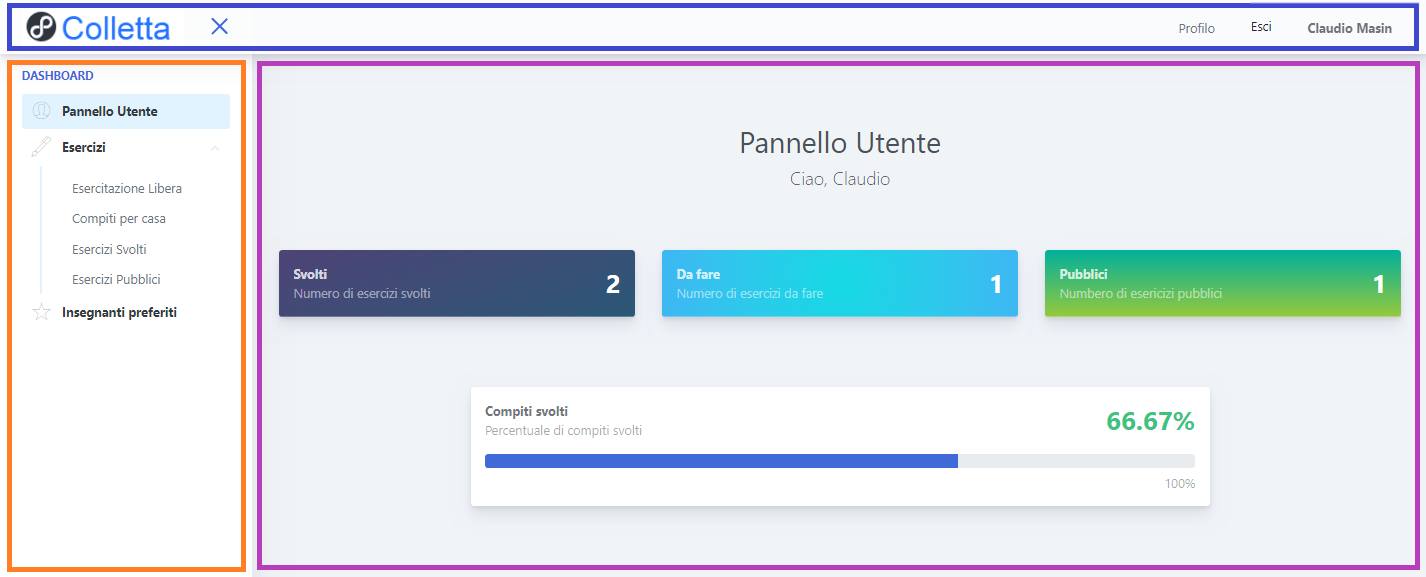
\includegraphics[width=17cm]{sez/img/istruzioni/panoramica.png} 
        \caption{Panoramica dell'interfaccia}\label{fig:1}
    \end{figure}
  La struttura generale di una pagina è la stessa per ogni utente loggato. Sono presenti i seguenti elementi di base:
    \begin{itemize}
        \item Barra del menu;
        \item {Sidebar}\ped{G};
        \item Contenuto della pagina.
    \end{itemize}
 A seconda del tipo di utente (Allievo, Insegnante, Sviluppatore, Amministratore) e della pagina selezionata, verranno visualizzati a schermo contenuti diversi. Ogni utente ha comunque a disposizione lo stesso header e un link al suo pannello utente.


\subsection{Utente non autenticato}
    \subsubsection{Registrazione}
    	\begin{figure}[H]
        	\centering
        	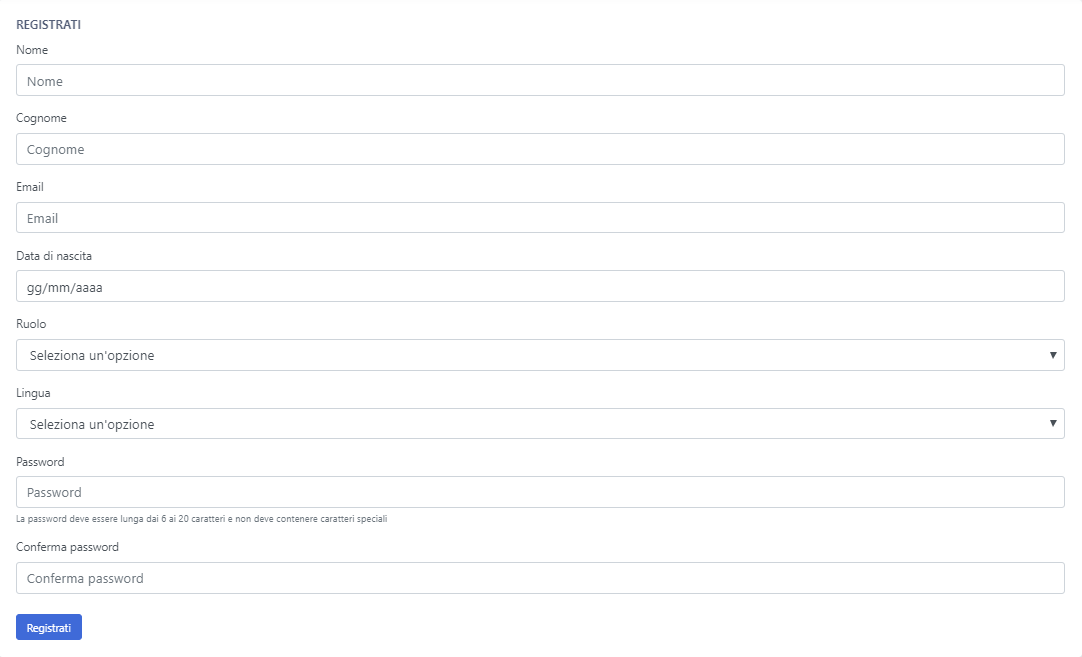
\includegraphics[width=1\linewidth]{sez/img/autenticazione/formRegistrazione.PNG} 
        	\caption{Form per la registrazione}\label{fig:registrazione}
    	\end{figure}
Se non si è ancora registrati è possibile farlo cliccando sul bottone \textit{Registrati} presente nella barra del menu. Una volta compilato il form viene inviata una mail per l'attivazione dell'account. E' necessario cliccare sul link appena ricevuto, successivamente verrà aperta una pagina con un messaggio di conferma. A questo punto se il ruolo scelto è \textit{Insegnante} o \textit{Allievo} è possibile accedere alla piattaforma; se \textit{Sviluppatore}, per poter accedere alla piattaforma è necessario attendere l'attivazione manuale da parte di un \textit{Amministratore} del sistema. I dati sono tutti obbligatori e il form visualizzato è quello in \autoref{fig:registrazione}.
    \subsubsection{Login}
    	\begin{figure}[H]
        	\centering
        	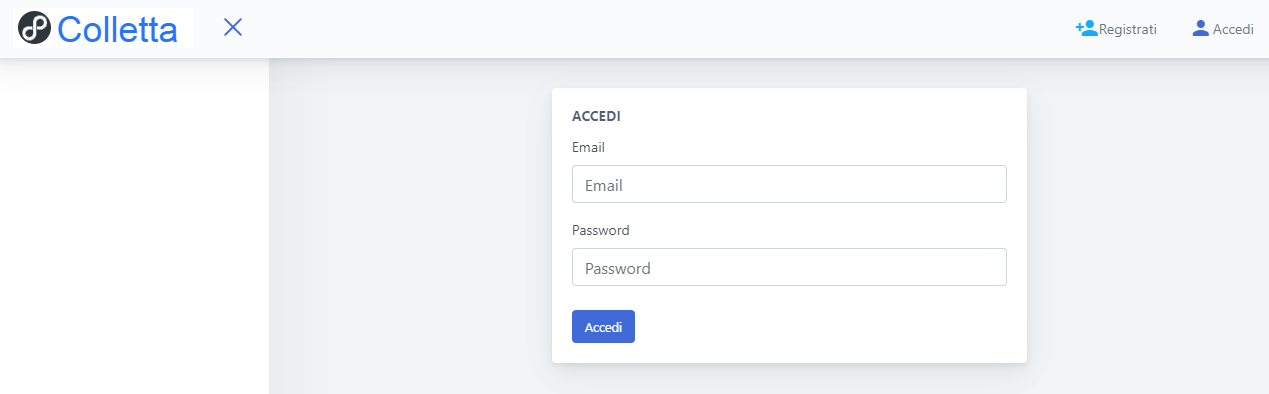
\includegraphics[width=1\linewidth]{sez/img/autenticazione/formAccedi.PNG} 
        	\caption{Form per effettuare il login}\label{fig:1}
    	\end{figure}
Una volta effettuata la registrazione, per poter accedere alla piattaforma è necessario recarsi sull'apposita pagina collegata dal link in altro a destra \textit{Accedi}, inserire l'email, la propria password e successivamente cliccare sul pulsante \textit{Accedi} del form.

    \subsubsection{Password dimenticata}
    	\begin{figure}[H]
        	\centering
        	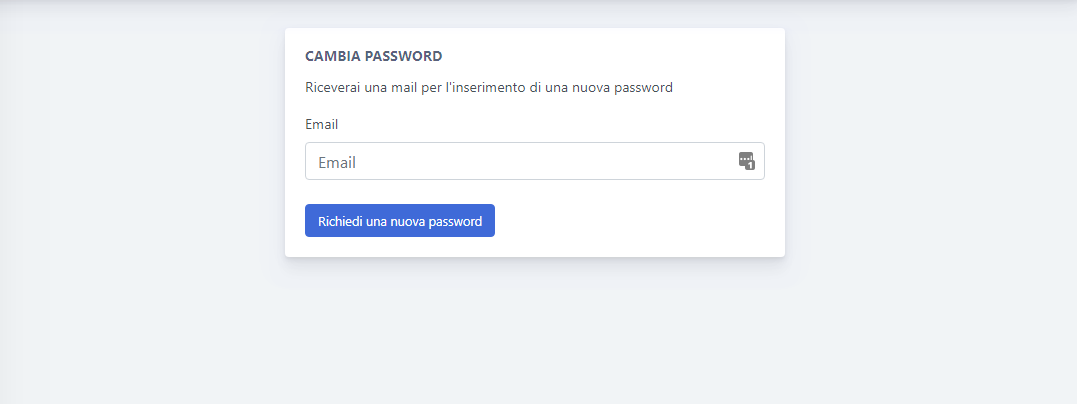
\includegraphics[width=1\linewidth]{sez/img/autenticazione/passwordDimenticata.png} 
        	\caption{Form per il recupero della password}\label{fig:1}
    	\end{figure}
	L'unico modo per cambiare la password di un utente iscritto alla piattaforma è  tramite il form di recupero password. Cliccando sul ling \textit{Password dimenticata?} presente all'interno del form di login, compare un form con una casella di testo per l'inserimento della mail utilizzata durante la registrazione. 
	
	Cliccando il pulsante \textit{Richiedi una nuova password}, se esiste effettivamente un account collegato a 	quella mail, viene inviata una mail contenente un link per l'inserimento della nuova password; cliccandolo verrà aperta una pagina della piattaforma \textit{Colletta} con un form contenente due caselle di testo per l'inserimento della nuova password.\\ Una volta inserita la nuova password è sufficiente cliccare il pulsante \textit{Cambia password}. Un messaggio di conferma indica che l'operazione è andata a buon fine.
\begin{figure}[H]
        	\centering
        	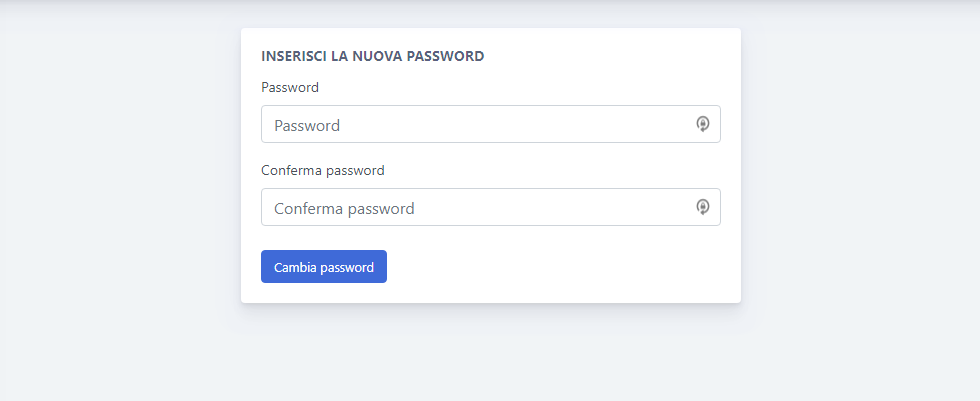
\includegraphics[width=1\linewidth]{sez/img/autenticazione/password.png} 
        	\caption{Form per l'inserimento della nuova password}\label{fig:1}
    	\end{figure}	
	
	
% UTENTE AUTENTICATO
\subsection{Utente autenticato generico}

    \subsubsection{Logout}
    Per effettuare il {logout}\ped{G} si deve cliccare sulla voce \textit{Esci} dalla barra del menu. Facendo ciò, l'utente termina la propria sessione.
    \subsubsection{Modifica dati}
    Cliccando su \textit{profilo} l'utente ha la possibilità visualizzare e modificare i propri dati tramite un form simile a quello di registrazione. L'utente non può modificare il proprio ruolo e la propria Email dopo l'iscrizione.

\newpage
    \subsection{Allievo}
      L'allievo si iscrive nel portale Colletta per svolgere esercizi di analisi grammaticale. Può svolgere esercizi assegnati da un'insegnante o svolgere esercizi liberi tramite il sistema di correzione automatica del sistema. L'allievo ha poi la possibilità di confrontare la sua soluzione con quella presentata dal sistema.
        \subsubsection{Sidebar}
          La sidebar dell'allievo presenta le seguenti voci:
            \begin{itemize}
                \item Pannello utente;
                \item Esercitazione libera;
                \item Compiti per casa;
                \item Esercizi svolti;
                \item Esercizi pubblici;
                \item Insegnanti preferiti.
            \end{itemize}
            

            
        \subsubsection{Pannello utente}
          Il pannello utente è un riassunto di tutti i progressi e le attività svolte dall'allievo. Al momento il pannello utente mostra un messaggio di benvenuto, l'allievo è quindi libero di selezionare una delle voci di menu ed esercitarsi.
%        	\begin{itemize}
%        		\item Progressi;
%        		\item Traguardi;
%        		\item Traguardo corrente;
%        		\item Prossimo traguardo;
%        		\item Valutazioni;
%        		\item Esercizi recenti;
%        		\item Insegnanti preferiti.
%        	\end{itemize}
        
        
               
	\newpage
        \subsubsection{Esercitazione libera}      
        	\begin{figure}[H]
                \centering
                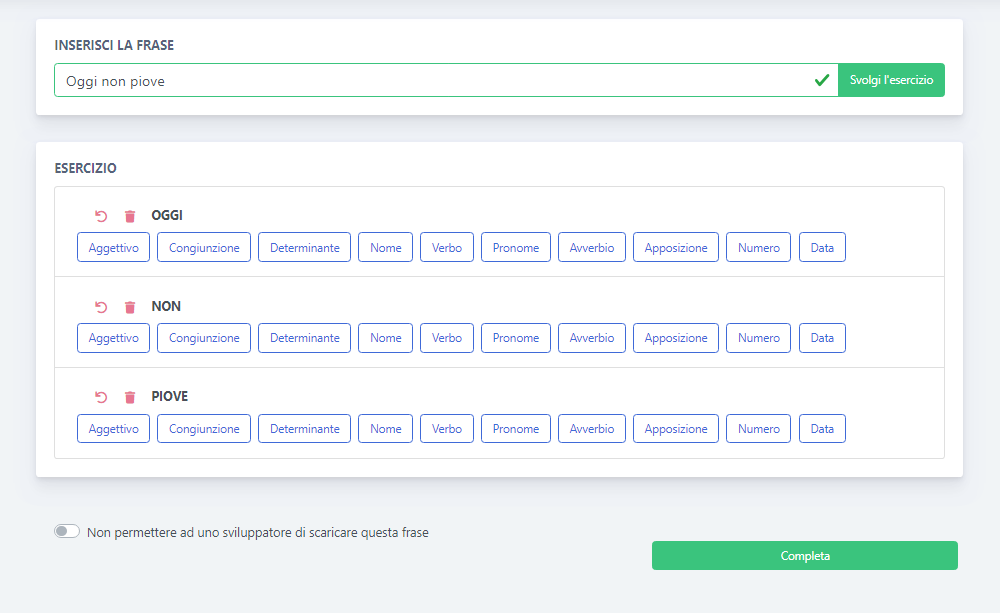
\includegraphics[width=17cm]{sez/img/studente/esercitazioneLiberaEsegui.PNG} 
                \caption{Svolgimento esercizio libero}\label{fig:1}
        	\end{figure}
          In questa pagina è possibile svolgere un esercizio inserendo nella casella di testo una frase da analizzare. La soluzione appena inserita viene confrontata con quella generata automaticamente.
        \\ Svolgimento:
        	\begin{enumerate}        
            	\item Scrivere la frase da analizzare all'interno della casella di testo;
            	\item Cliccare su \textit{Svolgi l'esercizio};
            	\item Svolgere l'esercizio e cliccare \textit{Completa}.
        	\end{enumerate}
        	\label{sec:esLib}
Lo svolgimento dell'esercizio è guidato; ogni pulsante rappresenta una scelta possibile, il primo pulsante selezionato corrisponde alla categorica alla quale appartiene la parola, le scelte successive raffinano l'analisi. Ad ogni click di un pulsante vengono generati dei pulsanti strettamente collegati a quello precedente. In caso non comparissero più pulsanti, significa che l'analisi per quella parola è terminata. In ogni momento l'allievo può decidere di resettare la soluzione per una determinata parola (icona cestino), o annullare l'ultima scelta (freccia indietro).        \linebreak	
        A sinistra del pulsante completa è presente un flag che indica se la frase appena inserita può essere messa a disposizione degli sviluppatori che utilizzano i dati della piattaforma; non selezionandolo si acconsente la condivisione di questo dato.
        	

        \newpage
  		\subsubsection{Compiti per casa}
 		  In questa sezione l'allievo ha la possibilità di visualizzare gli esercizi a lui assegnati e sceglierne uno da svolgere.
        	\begin{figure}[H]
            	\centering
            	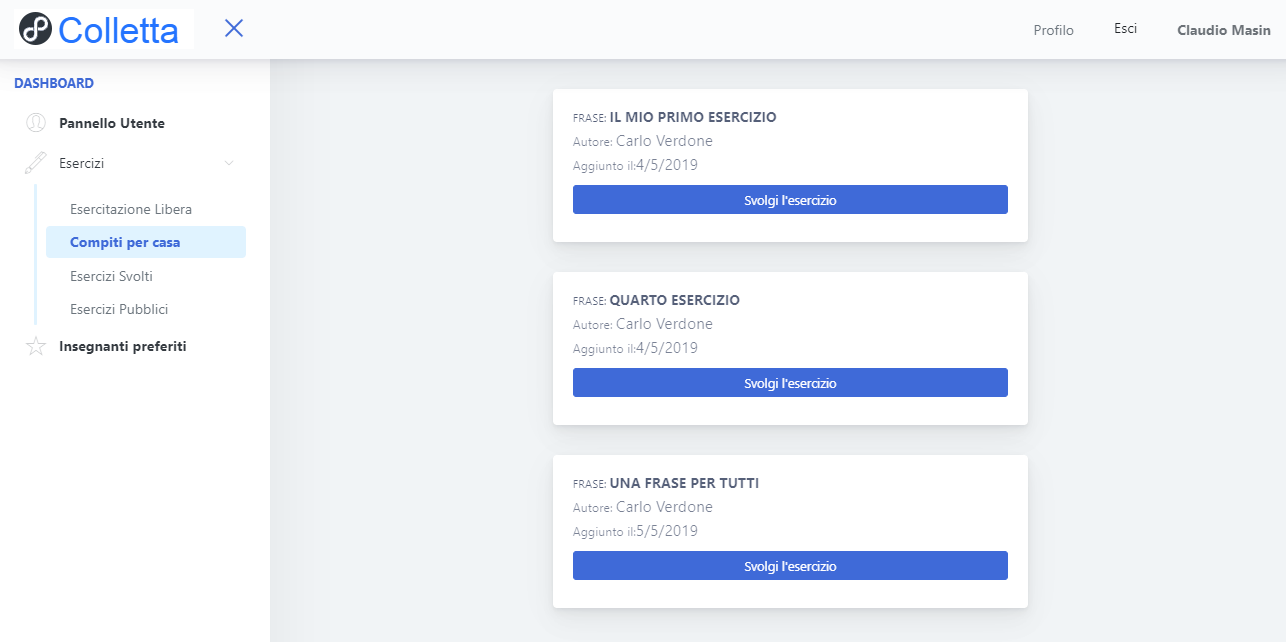
\includegraphics[width=17cm]{sez/img/studente/compitopercasa.PNG} 
            	\caption{Scelta esercizio da svolgere}\label{fig:1}
        	\end{figure}

		  L'allievo sceglie l'esercizio da svolgere tra quelli che sono stati assegnati cliccando su \textit{Svolgi l'esercizio}.   
       
        	\begin{figure}[H]
            	\centering
            	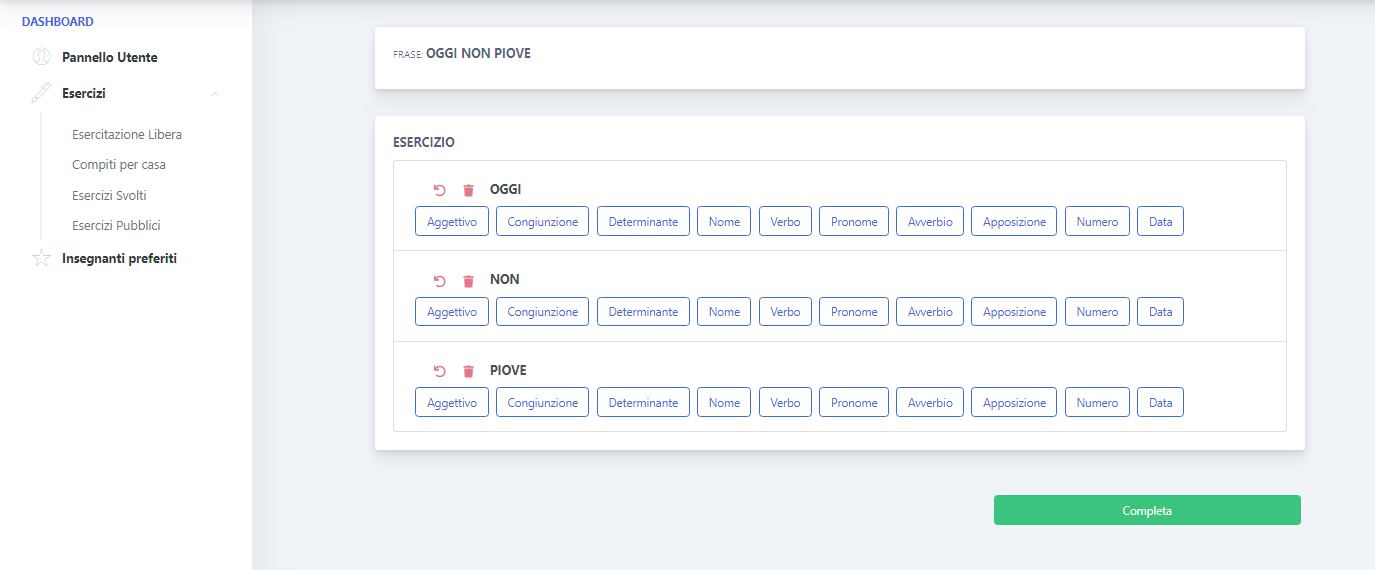
\includegraphics[width=17cm]{sez/img/studente/svolgimentoesercizio.PNG} 
            	\caption{Svolgimento esercizio}\label{fig:1}
        	\end{figure}      
	L'allievo esegue quindi l'analisi della frase allo stesso modo descritto in \S\ref{sec:esLib}. La soluzione visualizzata alla fine sarà in questo caso quella dell'insegnante che ha assegnato l'esercizio.
        
        
        \subsubsection{Esercizi svolti}
                 In questa pagina è possibile visualizzare lo storico degli esercizi che sono stati svolti. Per ogni esercizio svolto sono visualizzabili la data di aggiunta, la frase analizzata e il nome dell'insegnante che ha assegnato l'esercizio.
        	\begin{figure}[H]
            	\centering
            	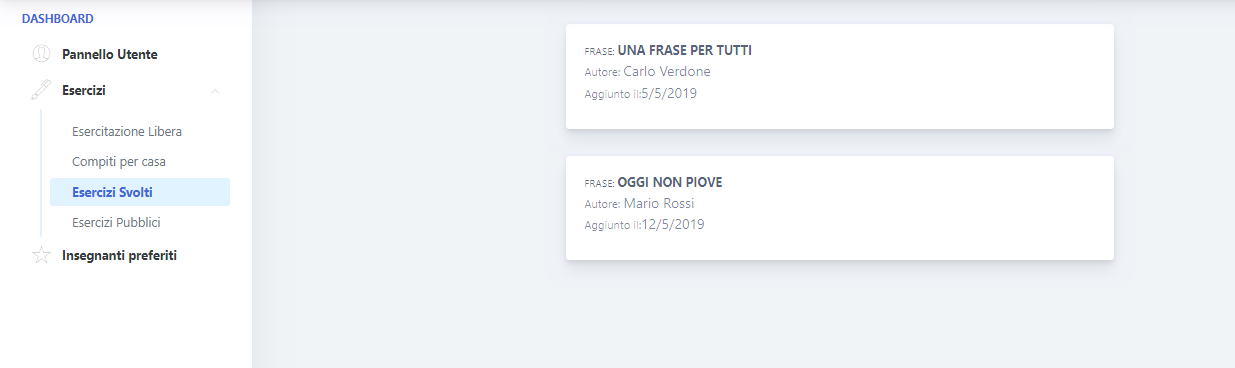
\includegraphics[width=17cm]{sez/img/studente/esercizisvolti.PNG} 
            	\caption{Storico esercizi svolti}\label{fig:1}
        	\end{figure}
          In questa pagina è possibile visualizzare lo storico degli esercizi che sono stati svolti. Per ogni esercizio svolto sono visualizzabili la data di aggiunta, la frase analizzata e il nome dell'insegnante che ha assegnato l'esercizio.
        
        
        
\subsubsection{Insegnanti preferiti}
        	\begin{figure}[H]
            	\centering
            	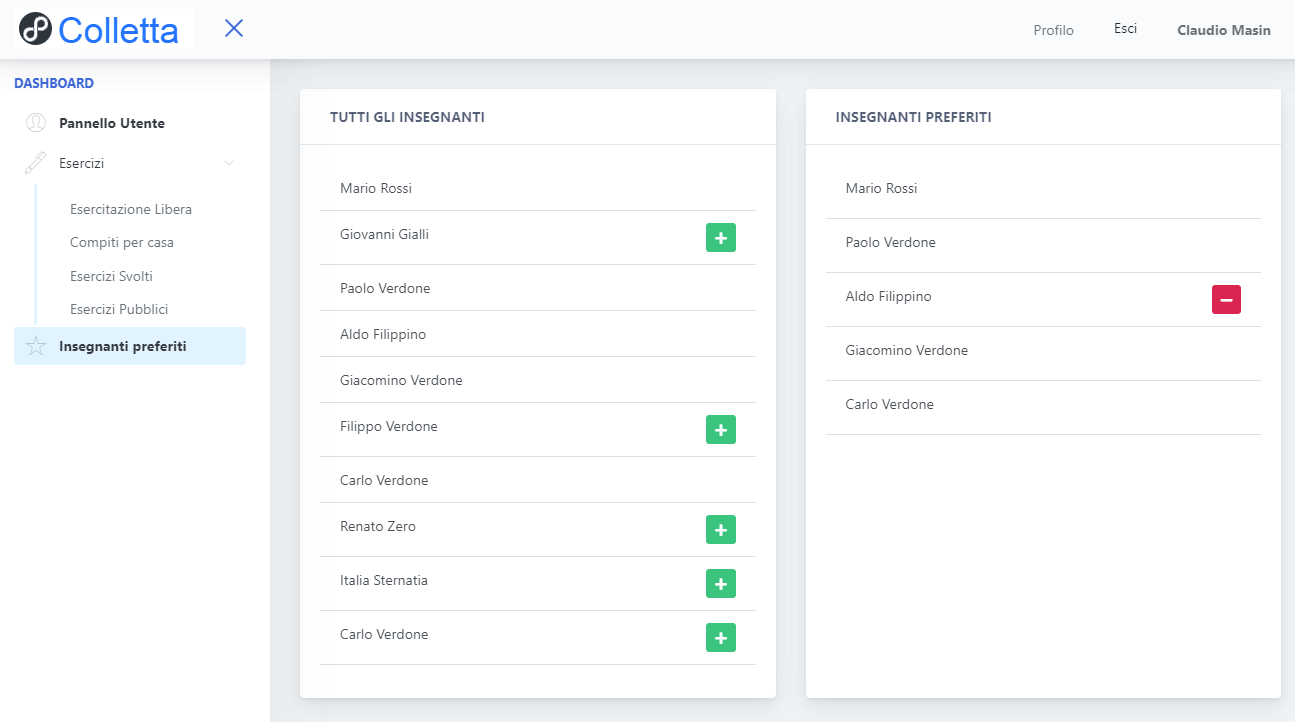
\includegraphics[width=17cm]{sez/img/studente/insegnantepreferito.png} 
            	\caption{Elenco insegnanti preferiti}\label{fig:1}
        	\end{figure}        
        In questa pagina troviamo l'elenco di tutti gli insegnanti presenti, nella lista di sinistra clicccando sul pulsante \textit{"+"} possiamo aggiungerli tra gli insegnanti preferiti, se invece si vuole rimuovere un insegnante dalla lista è sufficiente cliccare sul pulsante \textit{"-"} che compare se il cursore viene avvicinato al nome dell'insegnante che si vuole rimuovere.
        
        
        
\newpage
    \subsection{Insegnante}
      L'insegnante è l'utente che può inserire esercizi privati o decidere di assegnarli ai propri allievi. 
         \\La sidebar dell'insegnante presenta le seguenti voci:
        	\begin{itemize}
            	\item Pannello utente;
            	\item Inserisci esercizio;
            	\item Esercizi inseriti;
            	\item Gestione classi.
        	\end{itemize}
        
        
        
        \subsubsection{Pannello utente}
          Il pannello utente mostra un messaggio di benvenuto all'insegnante, che poi è libero di spostarsi sulla sidebar e assegnare esercizi ai propri allievi.
        
        
        \subsubsection{Inserisci esercizio}
          Questa sezione da la possibilità all'insegnante di inserire un esercizio nel sistema.
        	\begin{figure}[H]
            	\centering
        		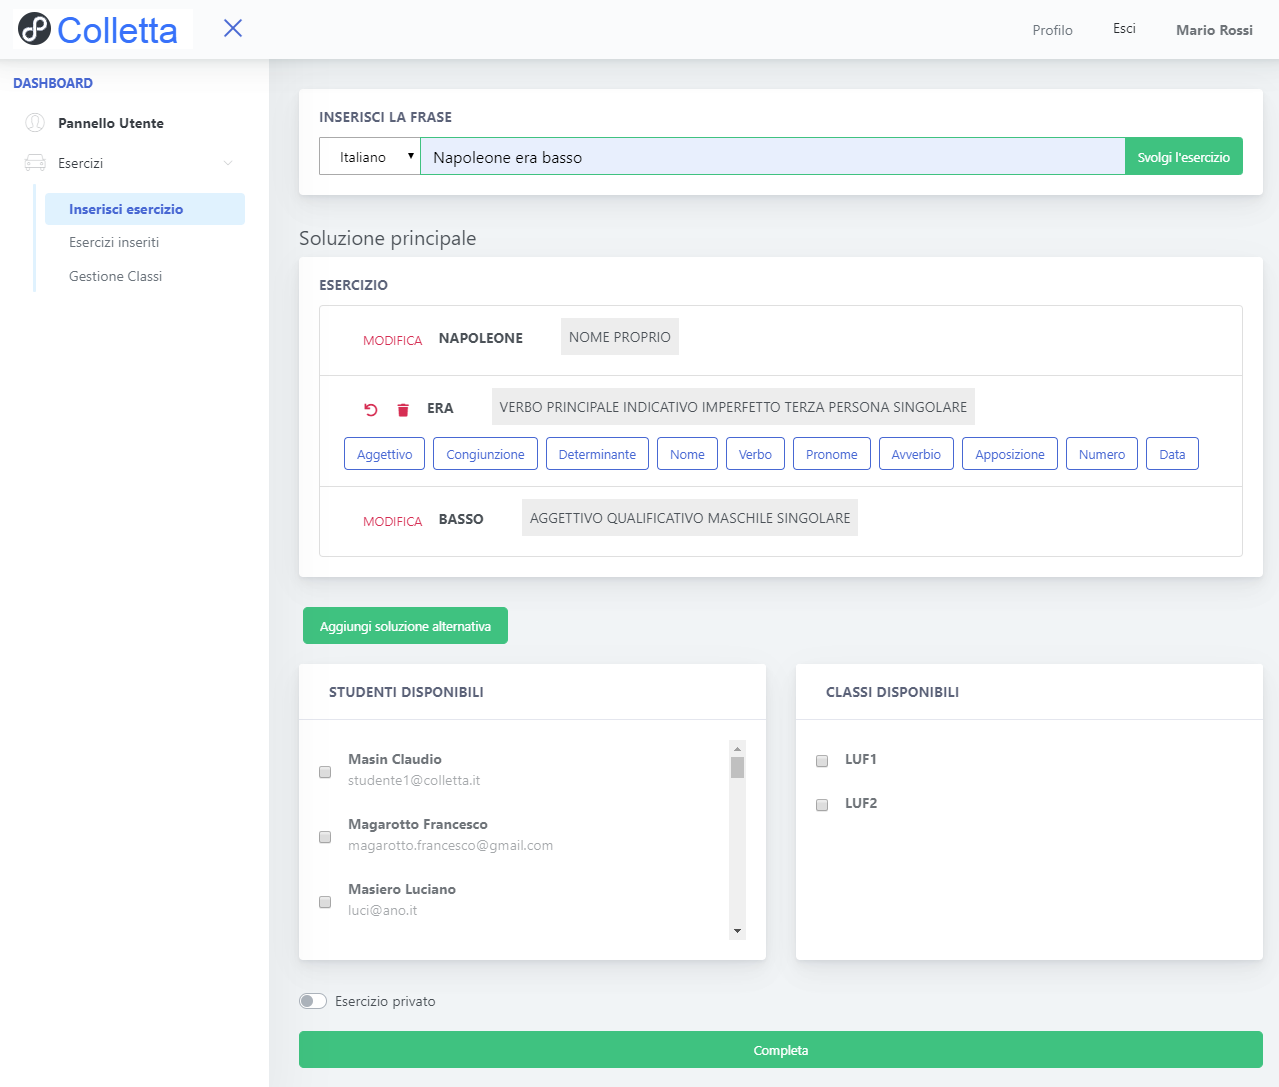
\includegraphics[width=17cm]{sez/img/insegnante/inserisciEsercizio.PNG} 
            	\caption{Inserimento e assegnazione esercizio}\label{fig:1}
        	\end{figure}
        
Dopo aver inserito la frase, verrà visualizzata la correzione automatica. Se ritenuta errata c'è la possibilità di modificare la soluzione cliccando su \textit{Modifica}. Durante lo svolgimento dell'esercizio l'insegnante ha la possibilità di tornare indietro di un passo, o di resettare completamente la soluzione per ogni parola. Questo processo è analogo a quello presentato in \S\ref{sec:esLib}. Finita la correzione, l'insegnate ha la possibilità di assegnare l'esercizio ad un singolo allievo, più allievi o una intera classe di allievi, e cliccando \textit{Completa} esso verrà aggiunto nel database.
        
         \begin{figure}[H]
            	\centering
        		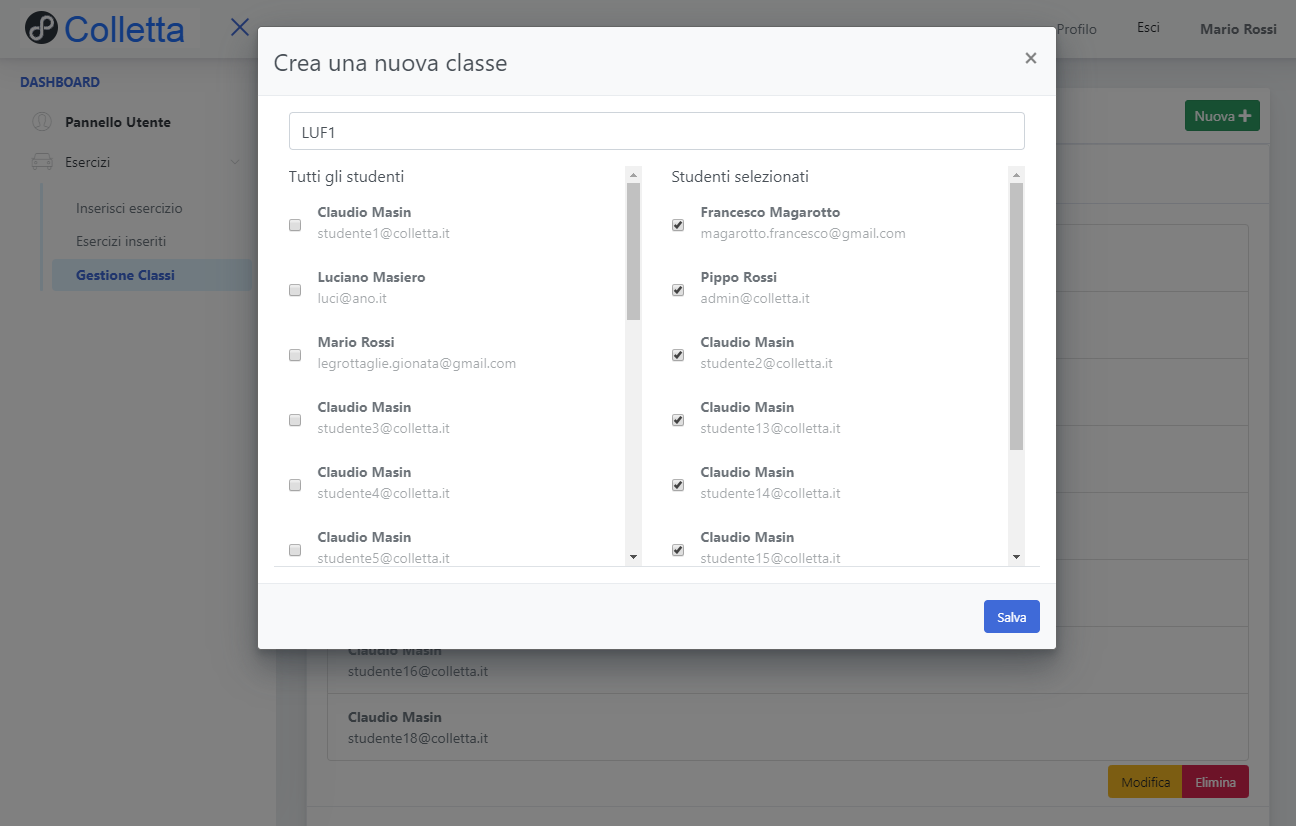
\includegraphics[width=17cm]{sez/img/insegnante/modificaclasse.PNG} 
            	\caption{Modifica una classe}\label{fig:1}
        	\end{figure}
        	
        	
Cliccando su \textit{Modifica} compare la finestra che ci permette di aggiungere nuovi allievi, rimuoverli o eventualmente modificare il nome. Per salvare le modifiche è sufficiente cliccare sul pulsante \textit{Salva}.
        
	\newpage
    \subsection{Sviluppatore}
    Lo sviluppatore compre un ruolo fondamentale all'interno della piattaforma. Egli è colui che utilizzerà i dati inseriti da \textit{Allievi} e \textit{Insegnanti}, con l'obiettivo di utilizzarli come input per i sistemi di autoapprendimento.
    Lo sviluppatore può iscriversi alla piattaforma utilizzando lo stesso sistema utilizzato dagli altri tipi di utenti a differenza dell'attivazione dell'account. E' necessario l'attivazione manuale da parte di un amministratore della piattaforma per poter accedere la prima volta. 
        	 \\Il pannello utente è l'unica pagina presente all'interno dell'area riservata di uno \textit{Sviluppatore}.
   
    	\subsubsection{Pannello utente}
    				\begin{figure}[H]
				\centering
				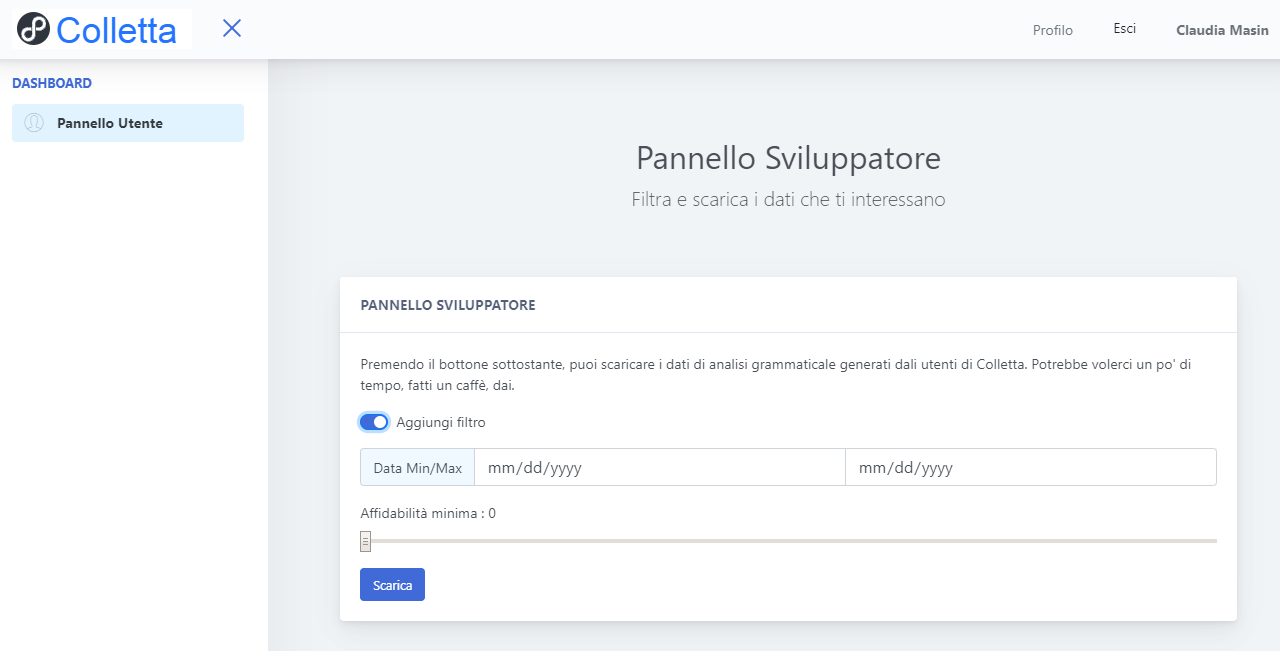
\includegraphics[width=17cm]{sez/img/sviluppatore/panelloutente.PNG}
				\caption{Pannello utente: Sviluppatore}\label{fig:1}
			\end{figure}
			 All'interno del pannello è presente un pulsante per scaricare tutti i dati presenti all'interno del sistema; eventualmente è possibile inserire dei filtri per avere dei dati che si avvicinano maggiormente alla proprie esigenze.
    	  Il pannello utente mostra un messaggio di benvenuto allo sviluppatore, che è libero di procedere allo scaricamento dei dati prodotti dagli utenti.
    	 Cliccando il flag \textit{Aggiungi filtro} compare un form contenente due caselle di testo per inserire un range di date in cui è stato inserito un esercizio e sotto di esso una barra di valori tra \textit{0 - 100} indicare l'affidabilità minima richiesta per una soluzione.
    	 Cliccando il pulsante \textit{Scarica} un file di formato {JSON}\ped{G} viene salvato all'interno della propria cartella predefinita dei download.

	\newpage
	\subsection{Amministratore}
	L'amministratore ha la possibilità di gestire tutti gli utenti che non siano amministratori, inoltre può approvare o declinare le richieste di iscrizione degli sviluppatori.
		  \\Voci nella sidebar:
			\begin{itemize}
				\item Pannello utente;
				\item Sviluppatori;
				\item Utenti.
			\end{itemize}



		\subsubsection{Pannello utente}
			\begin{figure}[H]
				\centering
				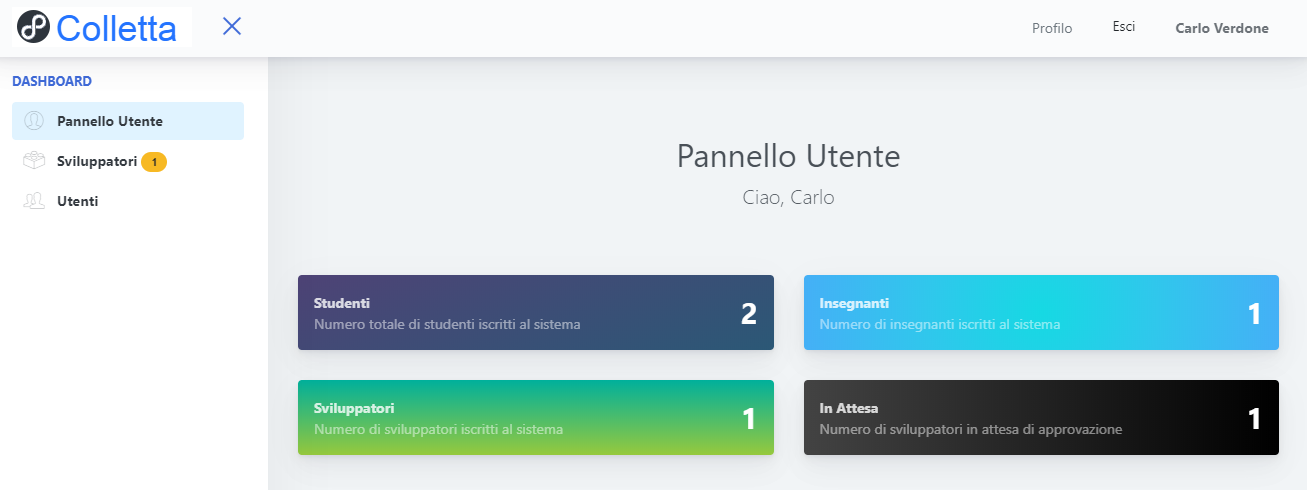
\includegraphics[width=17cm]{sez/img/amministratore/panelloadmin.PNG}
				\caption{Pannello utente: Amministratore}\label{fig:1}
			\end{figure}
		Il pannello utente contiene un breve riepilogo della situazione attuale all'interno della piattaforma.
		Sono presenti quattro box che indicano rispettivamente: il numero di \textit{Allievi} iscritti, il numero di \textit{Insegnanti} iscritti, il numero di \textit{Sviluppatori} iscritti ed approvati e il numero di \textit{Sviluppatori} iscritti ma ancora in attesa di approvazione.

		\subsubsection{Sviluppatori}
			\begin{figure}[H]
				\centering
				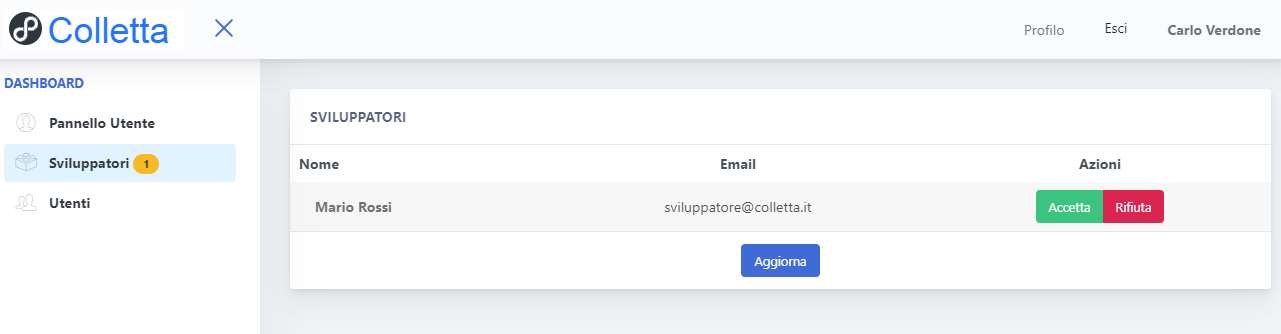
\includegraphics[width=17cm]{sez/img/amministratore/conf_ric_svil.PNG}
				\caption{Richieste di iscrizione degli sviluppatori}\label{fig:1}
			\end{figure}
		  In questa pagina l'amministratore può approvare o rifiutare le richieste di iscrizione degli sviluppatori. Viene presentata una lista contente gli sviluppatori che hanno richiesto di iscriversi al sistema. Ogni sviluppatore ha un nome e una mail. L'amministratore, premendo su \textit{Accetta}, consente allo sviluppatore di effettuare il login, premendo su \textit{Rifiuta} invece, rifiuta e cancella lo sviluppatore dal sistema. Premendo sul pulsante \textit{Aggiorna} viene ricaricata la lista degli \textit{Sviluppatori}.


		\subsubsection{Utenti}
			\begin{figure}[H]
				\centering
				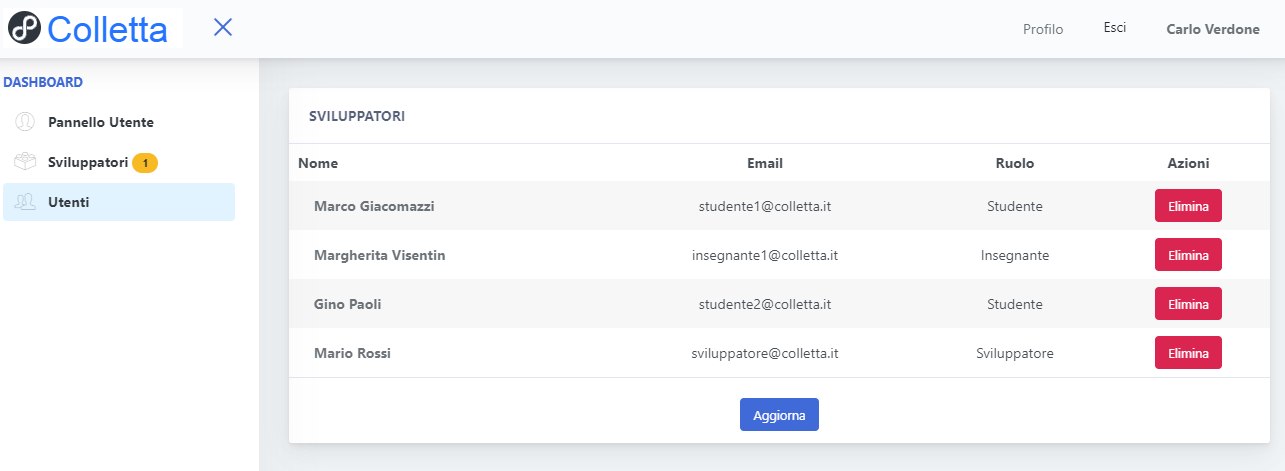
\includegraphics[width=17cm]{sez/img/amministratore/gestisciutenti.PNG}
				\caption{Gestione utenti}\label{fig:1}
			\end{figure}
		  In questa pagina l'amministratore può visualizzare gli utenti iscritti ed eventualmente eliminarli dal sistema. Per ogni utente sono presenti nome, email e ruolo (Insegnante, Sviluppatore o Allievi). Gli amministratori non figurano in questo elenco. 
		  
		  Cliccando su \textit{Elimina}, compare un alert per la conferma dell'eliminazione, cliccando su \textit{Si} l'utente viene eliminato, cliccando \textit{No} l'operazione viene annullata. Premendo su \textit{Aggiorna} la lista degli utenti viene aggiornata.
